%
% Course IFJ @ FIT VUT Brno, 2015
% IFJ15 Interpreter Project
%
% Authors:
% Lukas Osadsky  - xosads00
% Pavol Plaskon  - xplask00
% Pavel Pospisil - xpospi88
% Matej Postolka - xposto02

\documentclass[a4paper, 12pt]{article}

\usepackage[left=2cm,text={17cm, 24cm},top=3cm]{geometry}
\usepackage[czech]{babel}
\usepackage[utf8]{inputenc}
\usepackage[IL2]{fontenc}
\usepackage{times}
\usepackage{graphics}
\usepackage{url}
% START Pozadavky automatu
\usepackage{pgf}
\usepackage{tikz}
\usetikzlibrary{arrows,automata}
% END Pozadavky automatu
\pagenumbering{arabic}

\providecommand{\uv}[1]{\quotedblbase #1\textquotedblleft}

\begin{document}
%%%%%%%%%%%%%%%%%%%%%%%%%%%%%%%%%%%%%%%%%%%%%%%%
%               Title page
%%%%%%%%%%%%%%%%%%%%%%%%%%%%%%%%%%%%%%%%%%%%%%%%
\begin{titlepage}

\begin{center}
\fontsize{25}{20}\selectfont{\textsc{Vysoké učení technické v~Brně}}\\
\vspace{\stretch{0.0075}}
\fontsize{21}{0}\textsc{\selectfont{Fakulta informačních technologií}}\\
\vspace{\stretch{0.15}}
%Logo
\begin{figure}[ht]
    \begin{center}
        \scalebox{1}{\includegraphics{logo_bw.eps}}
    \end{center}
\end{figure}

\vspace{\stretch{0.2}}
\LARGE{Dokumentace IFJ15}\\
\Large{Tým \textit{052}, varianta \textit{a/2/II}}
\vspace{\stretch{0.618}}
\end{center}

\begin{large}
\begin{tabbing}
    Další členové: \quad \= Postolka Matej \quad \= xposto02 \quad \= 25 \%\kill
    Vedoucí týmu:  \> Postolka Matej \> xposto02 \> 25 \% \\
    Další členové: \> Osadský Lukáš  \> xosads00 \> 25 \% \\
             \> Plaskoň Pavol  \> xplask00 \> 25 \% \\
             \> Pospíšil Pavel \> xpospi88 \> 25 \% \\
\end{tabbing}
\end{large}

\end{titlepage}

%%%%%%%%%%%%%%%%%%%%%%%%%%%%%%%%%%%%%%%%%%%%%%%%
%                   Obsah
%%%%%%%%%%%%%%%%%%%%%%%%%%%%%%%%%%%%%%%%%%%%%%%%
\tableofcontents
\newpage
%%%%%%%%%%%%%%%%%%%%%%%%%%%%%%%%%%%%%%%%%%%%%%%%
%                   uvod
%%%%%%%%%%%%%%%%%%%%%%%%%%%%%%%%%%%%%%%%%%%%%%%%
\section{Práce v týmu}
+ vývojový cyklus? speciální techniky
\section{Lexikální analyzátor} \label{lexer}
\subsection{Diagram konečného automatu lexikálního analyzátoru}

% ****************************************

\begin{center}
\begin{tikzpicture}[scale=0.2]
\tikzstyle{every node}+=[inner sep=0pt]
\draw [black] (21.7,-65.3) circle (3);
\draw (21.7,-65.3) node {$start$};
\draw [black] (43,-35.5) circle (3);
\draw (43,-35.5) node {$-$};
\draw [black] (43,-42.1) circle (3);
\draw (43,-42.1) node {$/$};
\draw [black] (43,-48.8) circle (3);
\draw (43,-48.8) node {$+$};
\draw [black] (43,-55.3) circle (3);
\draw (43,-55.3) node {$*$};
\draw [black] (43,-61.9) circle (3);
\draw (43,-61.9) node {$<$};
\draw [black] (43,-69.7) circle (3);
\draw (43,-69.7) node {$($};
\draw [black] (43,-76.3) circle (3);
\draw (43,-76.3) node {$>$};
\draw [black] (43,-82.8) circle (3);
\draw (43,-82.8) node {$)$};
\draw [black] (43,-89.5) circle (3);
\draw (43,-89.5) node {$=$};
\draw [black] (43,-96.2) circle (3);
\draw (43,-96.2) node {$!$};
\draw [black] (43,-102.7) circle (3);
\draw (43,-102.7) node {$\{$};
\draw [black] (43,-109.3) circle (3);
\draw (43,-109.3) node {$\}$};
\draw [black] (43,-116) circle (3);
\draw (43,-116) node {$,$};
\draw [black] (43,-122.7) circle (3);
\draw (43,-122.7) node {$;$};
\draw [black] (43,-129.3) circle (3);
\draw (43,-129.3) node {$eof$};
\draw [black] (53.7,-67.6) circle (3);
\draw (53.7,-67.6) node {$"$};
\draw [black] (21.137,-62.355) arc (-172.77362:-258.33811:23.919);
\fill [black] (40.03,-35.92) -- (39.15,-35.59) -- (39.35,-36.57);
\draw (24.82,-44.06) node [left] {$-$};
\draw [black] (21.688,-62.302) arc (-183.74044:-261.36985:21.614);
\fill [black] (40.01,-42.34) -- (39.15,-41.97) -- (39.3,-42.96);
\draw (26.8,-47.63) node [left] {$/$};
\draw [black] (22.706,-62.476) arc (156.60402:98.92214:22.694);
\fill [black] (40.01,-49.07) -- (39.15,-48.7) -- (39.3,-49.69);
\draw (28.57,-53.05) node [above] {$+$};
\draw [black] (23.632,-63.007) arc (136.44053:93.85804:24.903);
\fill [black] (40,-55.32) -- (39.17,-54.88) -- (39.24,-55.87);
\draw (30.11,-57.12) node [above] {$*$};
\draw [black] (24.417,-64.029) arc (112.53366:85.60493:33.937);
\fill [black] (40.02,-61.54) -- (39.26,-60.98) -- (39.19,-61.98);
\draw (31.64,-61.26) node [above] {$<$};
\draw [black] (40.192,-75.245) arc (-111.54859:-123.07796:89.674);
\fill [black] (40.19,-75.25) -- (39.63,-74.49) -- (39.26,-75.42);
\draw (30.92,-72.02) node [below] {$>$};
\draw [black] (40.425,-81.261) arc (-121.90507:-136.90772:82.857);
\fill [black] (40.43,-81.26) -- (40.01,-80.41) -- (39.48,-81.26);
\draw [black] (40.638,-87.65) arc (-129.1442:-148.14957:79.776);
\fill [black] (40.64,-87.65) -- (40.33,-86.76) -- (39.7,-87.53);
\draw (30.57,-79.94) node [left] {$=$};
\draw [black] (40.777,-94.185) arc (-133.32547:-157.51596:75.618);
\fill [black] (40.78,-94.19) -- (40.54,-93.27) -- (39.85,-94);
\draw (29.8,-83.45) node [left] {$!$};
\draw [black] (40.736,-100.732) arc (-132.41049:-168.26487:60.719);
\fill [black] (40.74,-100.73) -- (40.48,-99.82) -- (39.81,-100.56);
\draw (28.27,-87.17) node [left] {$\{$};
\draw [black] (40.663,-107.42) arc (-130.41558:-177.92202:53.951);
\fill [black] (40.66,-107.42) -- (40.38,-106.52) -- (39.73,-107.28);
\draw (26.38,-90.93) node [left] {$\}$};
\draw [black] (40.809,-113.951) arc (-134.42097:-180.00269:63.915);
\fill [black] (40.81,-113.95) -- (40.59,-113.03) -- (39.89,-113.75);
\draw (25.88,-93.99) node [left] {$,$};
\draw [black] (40.676,-120.803) arc (-130.69976:-188.58246:57.915);
\fill [black] (40.68,-120.8) -- (40.4,-119.9) -- (39.74,-120.66);
\draw (23.39,-97.85) node [left] {$;$};
\draw [black] (40.761,-127.304) arc (-133.03769:-190.14614:65.115);
\fill [black] (40.76,-127.3) -- (40.52,-126.39) -- (39.83,-127.12);
\draw (22.65,-100.97) node [left] {$eof$};
\draw [black] (40.012,-69.434) arc (-96.13723:-107.20593:81.86);
\fill [black] (40.01,-69.43) -- (39.27,-68.85) -- (39.16,-69.85);
\draw (31.72,-68.78) node [below] {$($};
\draw [black] (24.694,-65.118) arc (92.69275:79.08513:110.303);
\fill [black] (50.76,-66.99) -- (50.07,-66.35) -- (49.88,-67.33);
\draw (37.88,-64.72) node [above] {$"$};
\draw [black] (18.798,-64.586) arc (283.89909:-4.10091:2.25);
\draw (15.99,-59.51) node [left] {$white\mbox{ }space$};
\fill [black] (20.5,-62.56) -- (20.8,-61.67) -- (19.82,-61.91);
\draw [black] (11.9,-65.3) -- (18.7,-65.3);
\fill [black] (18.7,-65.3) -- (17.9,-64.8) -- (17.9,-65.8);
\end{tikzpicture}
\end{center}
% ****************************************
\begin{figure}%[ht]
    \begin{center}
        \scalebox{0.9}{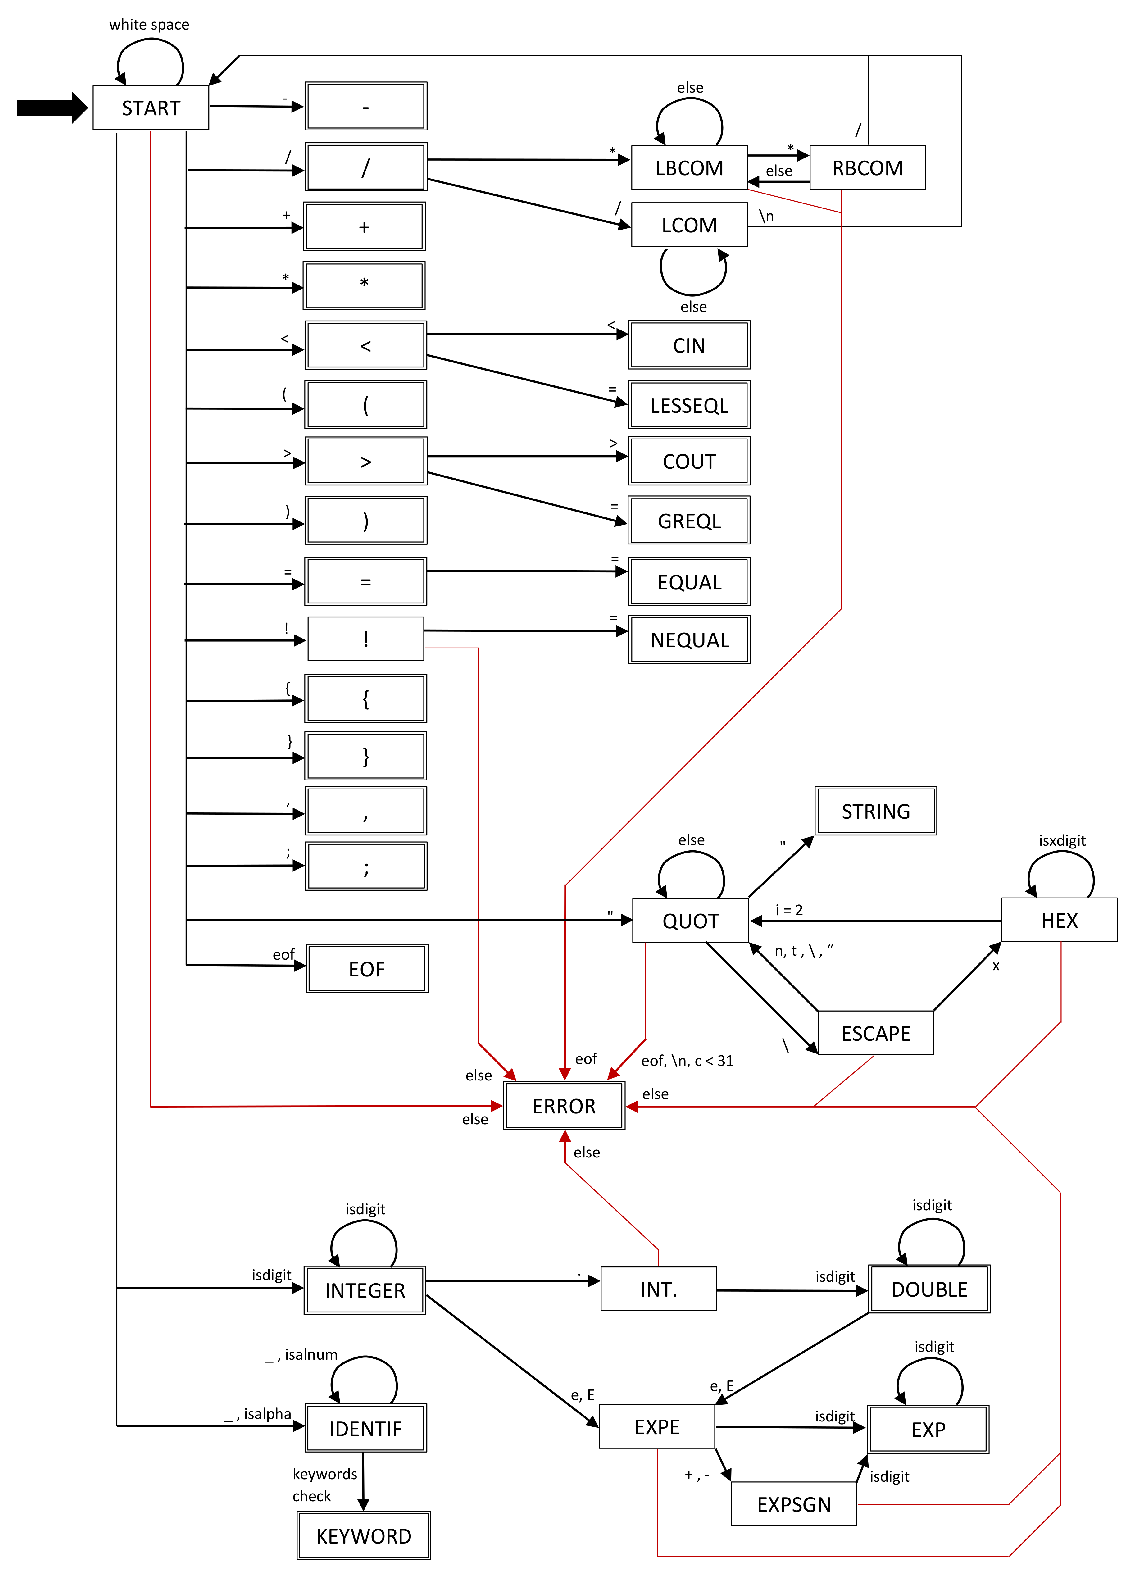
\includegraphics{lex.eps}}
    \end{center}
\end{figure}
% ****************************************

\section{Syntaktický analyzátor} \label{parser}
\subsection{LL gramatika}
Dodá Matěj
\begin{verbatim}
IFJ15 LL GRAMMAR RULES
<PROG>=<FUNCTION_DECL><PROG>
<FUNCTION_DECL>=<DATA_TYPE>t_identifier(<FUNC_DECL_PARAMS>)<NESTED_BLOCK>
<DATA_TYPE>t_int
<DATA_TYPE>t_double
<DATA_TYPE>t_string
<DATA_TYPE>t_auto
<FUNC_DECL_PARAMS>
\end{verbatim}
\section{Interpret} \label{interpret}

\subsection{Řadíci algoritmus -- Heap Sort}
Funkce pro seřazení prvků v poli.

\subsection{Vyhledávaní podřetězce -- Knuth-Morris-Pratt}
Vyhledání podřetězce v řetězci ve vestavěné funkci \texttt{find} je řešeno
algoritmem Knuth-Morris-Pratt. Základem algoritmu je vytvoření masky, tzv.
\texttt{Fail vector}. Je to pole celých čísel o délce hledaného textu. Ke
každému písmenu hledaného řetězce je přiřazeno číslo, které určuje index, kam
se má program vrátit v případě neshody znaků.

\subsection{Tabulka s rozptýlenými položkami}
Datová struktura použitá pro tabulky symbolů. Výhodou je rychlost vyhledávání
položek. Základem je pole ukazatelů na
jednotlivé položky. Položky obsahují svůj klíč, data a ukazatel na další
položku, aby mohly být propojené v jednosměrně vázaný lineární
seznam (seznam synonym). V případě ideální hashovací funkce není propojení v
seznam potřebné, čas přístupu k položkám konstantní. Nalezení takové
funkce je ale problematické. V případě konfliktů se čas nalezení položky
prodloužuje o prohledání lineárního seznamu.

\section{TODO} \label{todo}
+kontrola čitelnosti a komentovanosti kódů, zdroje! (např. odkud prvočísla do hash tabulky)
\end{document}

